\documentclass[../main.tex]{subfiles}
 
\begin{document}

\subsection{ Main Decoding Processes }



\subsection{Prediction overview}

The prediction methods may have a great influence on the compression performance.H.264 supports two prediction options: \textbf{Intra prediction} using data within
the current frame, \textbf{Inter prediction} using motion compensated prediction from previously
coded frames. H.264 provides multiple prediction block sizes, multiple reference frames and special modes. All these features give H.264 a great deal of flexibility in the prediction process. By selecting the best prediction options for an individual macroblock, H.264 can minimize the residual size to produce a highly compressed bitstream.

\subsubsection{ Macroblocks and Further Block Division }

\subsubsection{ Intra-Prediction }


   \begin{figure} [ht]
   \begin{center}
   \begin{tabular}{c} %% tabular useful for creating an array of images 
   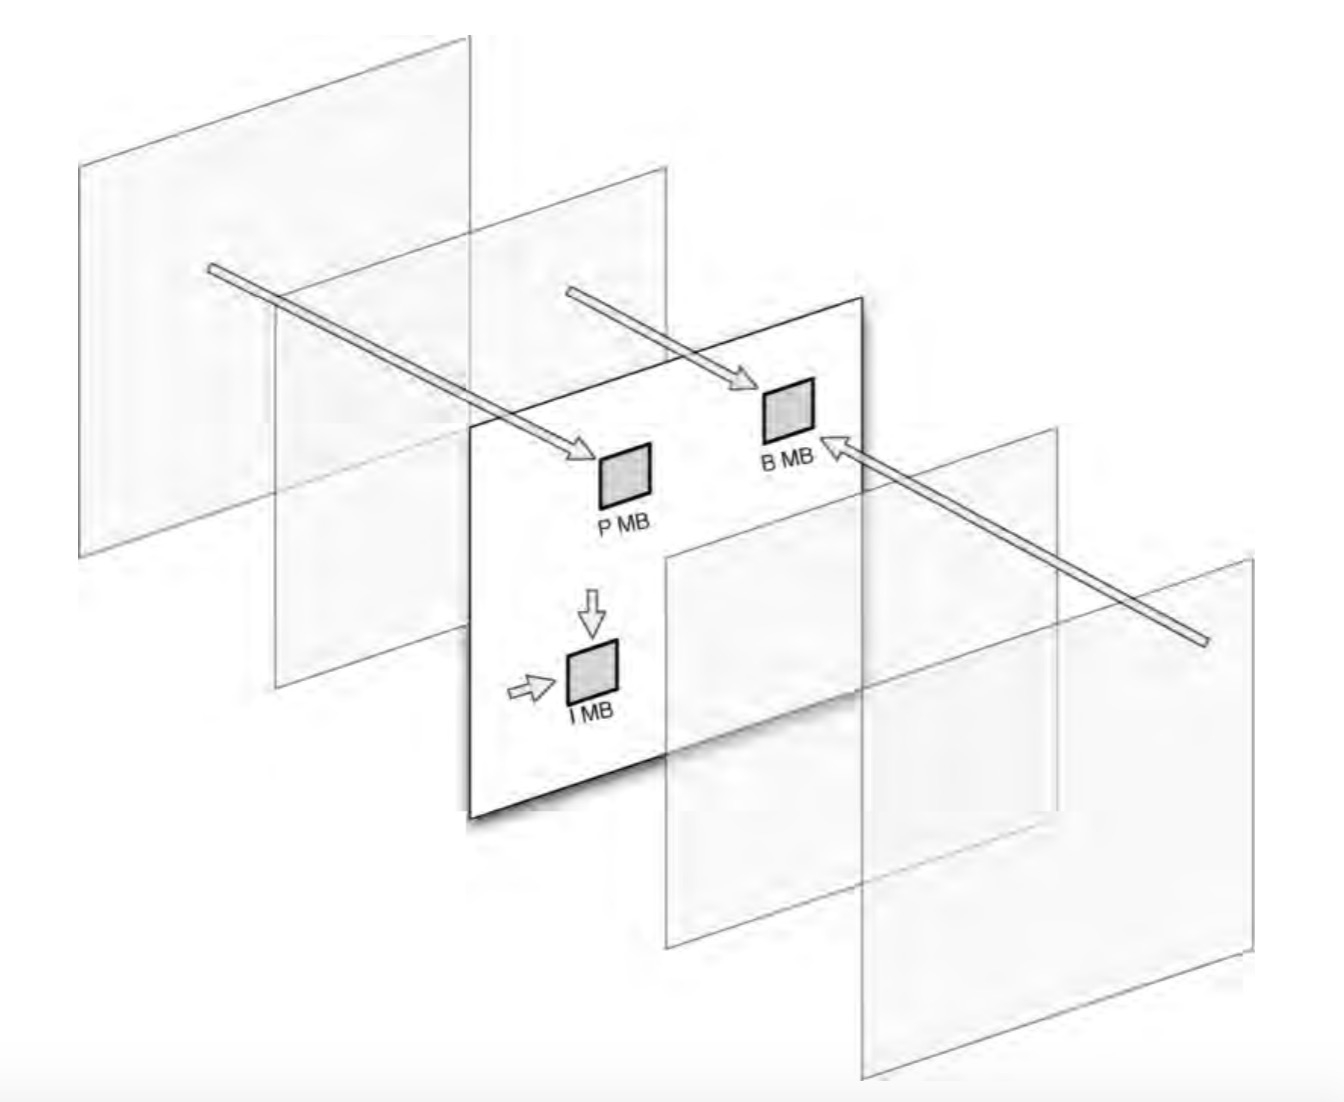
\includegraphics[height=5cm]{marcoblock.jpg}
   \end{tabular}
   \end{center}
   \caption[example] 
%>>>> use \label inside caption to get Fig. number with \ref{}
   { \label{fig:example} 
Marcoblock}
   \end{figure}     % 在reference中引用
   
\subsubsection{ Inter-Prediction }

Inter prediction is the process of predicting
a block of luma and chroma samples from a reference picture that has
previously been coded and transmitted. It
takes advantage of the fact that the content of a new frame in
the video often has high correlation to the data in the
previous frames.The offset between the position of the current partition and the prediction
region in the reference picture is a motion vector. The motion vector may point to integer,
half- or quarter-sample positions in the luma component of the reference picture. 

The decoded pictures stored in the Decoded
Picture Buffer (DPB), in which case they may be used as
reference pictures for inter prediction.The pictures in the DPB are listed in a particular order, and
the list can be classified into three different types:

\begin{table}[ht]
\label{tab:list}
\begin{center}       
\begin{tabular}{|l|l|} 
\hline
\rule[-1ex]{0pt}{3.5ex}  List0 (P slice) & A single list of all the reference pictures.  By default, the first picture in
the List is the most recently decoded picture.\\  %表格内容需换行
\hline
\rule[-1ex]{0pt}{3.5ex}  List0 (B slice) & A list of all the reference pictures. By default, the first picture in the List
is the picture \textbf {before} the current picture in display order.   \\%表格内容需换行
\hline
\rule[-1ex]{0pt}{3.5ex}  List1 (B slice) & A list of all the reference pictures. By default, the first picture in the List
is the picture \textbf {after} the current picture in display order.  \\%表格内容需换行
\hline

\end{tabular}
\end{center}
\caption{Three types of DPB list} 
\end{table}

Each $16 \times 16$ P or B macroblock may be predicted using a range
of block sizes. The macroblock is split into one, two or four
macroblock partitions:
(a) one $16 \times 16$ macroblock partition 
(b) two $8 \times 16$ partitions
(c) two $16 \times 8$ partitions or
(d) four $8 \times 8$ partitions.If $8 \times 8$ partition size is chosen, then each $8 \times 8$ block of luma samples and associated chroma
samples, a sub-macroblock, is split into one, two or four sub-macroblock partitions): one
8 × 8, two 4 × 8, two 8 × 4 or four 4 × 4 sub-MB partitions

\begin{figure} [ht]
   \begin{center}
   \begin{tabular}{c} %% tabular useful for creating an array of images 
   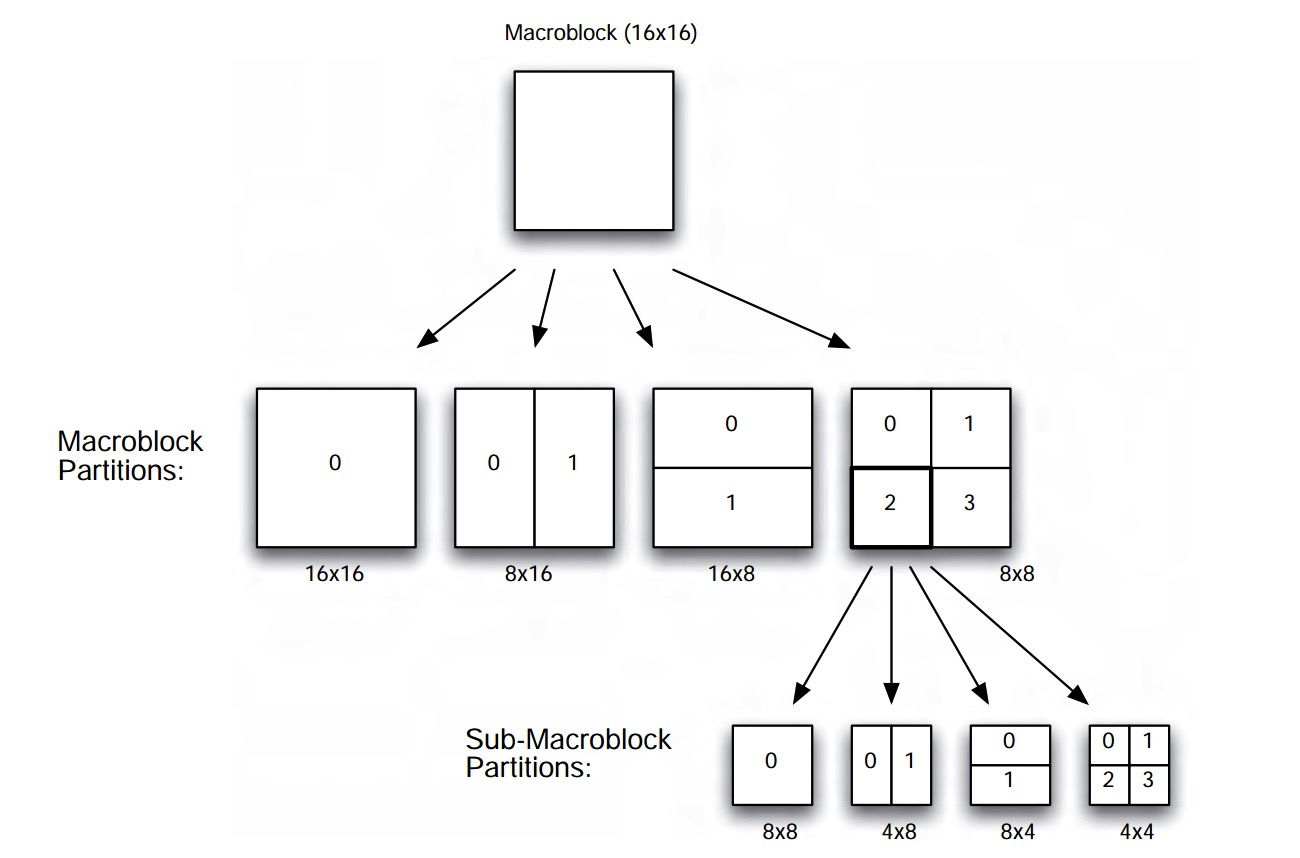
\includegraphics[height=10cm]{marcoblockpartition.jpg}
   \end{tabular}
   \end{center}
   \caption[example] 
%>>>> use \label inside caption to get Fig. number with \ref{}
   { \label{fig:example1} 
Macroblock partitions and sub-macroblock partitions}
   \end{figure}     % 在reference中引用
   
Each macroblock partition and sub-macroblock partition has one or two motion vectors
(x, y), each pointing to an area of the same size in a reference frame that is used to predict the
current partition. 
Motion vectors for neighboring partitions are often highly
correlated and so each motion vector is predicted from vectors of nearby, previously coded
partitions. 








\end{document}